% !TeX program = lualatex
\chapter{Ergebnisse} % Main chapter title
\label{Results} % For referencing the chapter elsewhere, use \ref{Results}
Anhand der Expertenbefragungen konnten insgesamt zwölf verschiedene Kategorien zu den jeweiligen Sichtweisen der einzelnen Stakeholder herausausgearbeitet werden. Unterschieden wird hierbei zwischen Kategorien mit einstimmigen und abweichenden Ergebnissen, wobei die genaue Bedeutung dieser Eigenschaften in den entsprechenden Kapiteln näher erläutert werden.
Die Alternativen zu den einzelnen Aspekten, welche von den einzelnen Stakeholdern vorgeschlagen wurden, werden darauffolgend aufgelistet. Als Letztes werden die vorgeschlagenen Alternativen in Bezug auf die Existenz, Verarbeitung und Auswertung der persönlichen Daten, welche die Stakeholder im Verlauf der Befragungen genannt haben, vorgestellt.

\section{Kategorien mit einstimmigen Ergebnissen} \label{clearresult}
In diesem Kapitel werden die einzelnen Kategorien anhand der Einstimmigkeit der einzelnen Kategorien aufgelistet. Einstimmig bedeutet in diesem Fall, dass bei den einzelnen Kategorien eine Abweichung von maximal drei von sieben Befragten (<50\%) stattgefunden hat - also anhand
der absoluten Häufigkeit eine eindeutige Aussage getroffen werden kann. \newline 
Hierbei wird zwischen der Präferenz der Privatsphäre im Allgemeinen oder der Benutzerfreundlichkeit bzw. Einfachheit unterschieden: Kategorien, in welchen Experten überwiegend
(>50\% der Experten sind der selben Ansicht) angegeben haben, die Privatsphäre sei ihnen wichtiger, werden dem Kapitel \ref{privacy} zugeordnet, wohingegen die Kategorien, in welchen die Privatsphäre
aufgrund der Benutzerfreundlichkeit und Einfachheit vernachlässigt wurde, dem Kapitel \ref{noprivacy} zugerechnet werden.
\subsection{Kategorien mit einer Präferenz für die Benutzerfreundlichkeit und Einfachheit} \label{noprivacy}
\textbf{Verarbeitete Daten zur Unterstützung der Softwareentwicklung in DevOps-Tools:} \newline
Zu Beginn der Interviews haben alle Befragten angegeben, mit persönlichen Daten in Berührung zu kommen und diese auch zu verarbeiten. Dabei haben alle vier Softwareentwickler angegeben, die Nutzeraktivitäten und den Programmcode von Kollegen 
einsehen und verarbeiten zu können. Diese genannten Daten beinhalten Benutzernamen, Zeitstempel (in Git Commits, Builds und Deployments, z.T.).
Erfolgen tue dies zur Nachvollziehbarkeit der Builds und Deployments, des Programmcodes selbst, z.B. durch Git Commits und zur allgemeinen Fehlerbehebung bei fehlgeschlagenen Builds bzw. fehlerhaftem Programmcode. 
Zwei Befragte haben zudem angegeben, Zugriff auf sensible Kundendaten in Form von Klarnamen, Anschriften, E-Mail Adressen o.Ä. zu besitzen: Dies ist bei jenen der Fall, welche häufig mit externen Ansprechpartnern und Unternehmen in Kontakt treten 
und zusammenarbeiten müssen. \newline \newline
\textbf{Bevorzugter Detailgrad von Zeitstempeln in DevOps-Tools:} \newline
Dieser Aspekt nimmt genaueren Bezug auf Zeitstempel in DevOps-Tools und befasst sich mit der Auflösung (z.B. Detailgrad, Lebensdauer und relevante Faktoren) dieser. Hier wurden die Experten befragt, in welcher Auflösung diese konkret den Zeitstempel 
im Arbeitsalltag benötigen. Bis auf eine Ausnahme, haben alle Befragten angegeben, einen konkreten Zeitstempel mit der Anfangs- und Endzeit (bzw. alternativ mit der Anfangszeit und der Dauer) zu benötigen und auf diesen nicht verzichten zu können. Dies sei
vor allem in der Fehlerbehebung (z.B. von fehlerhaften Commits) elementar, denn nur durch eine genaue Zeitangabe könne man den Fehler in Logs, im Code selbst (\enquote{Wie lange hat es gedauert, bis der Fehler aufgetreten ist?}) oder bei potenziellen Verantwortlichen 
suchen. \newline \newline
\textbf{Allgemeine Auswertungen von persönlichen Daten aus DevOps-Tools:} \newline
Bei dieser Frage sollten die Befragten angeben, ob diese sich Auswertungsmöglichkeiten von persönlichen Daten aus DevOps-Tools vorstellen könnten, welche sie selbst nicht zwangsläufig durchführen, aber welche bei anderen Kollegen bzw. Unternehmen
zum Einsatz kommen könnten. Hier haben alle Stakeholder angegeben, dass unter großer Wahrscheinlichkeit eine Form der Leistungsbeurteilung bzw. -bewertung stattfinden könnte. Da in der Regel Benutzernamen und Zeitstempel in Builds, (Git) Commits und gelegentlich auch in Log-Dateien vorzufinden sind, könne man
anhand dieser Daten Rückschlüsse auf die Quantität und Qualität der einzelnen Faktoren ziehen. \newline Ein Experte hat zudem angegeben, dass in seinem eigenen Unternehmen diese Daten häufig zum Einsatz zur Problembehebung kommen: Dabei wird anhand des Benutzernamens und Zeitstempels die Person hinter einem Build,
einem Git Commit oder einer anderen Ausführung ermittelt und durch gemeinsame Absprache mit diesem, eine Behebung des Problems angesteuert. \newline Ein weiterer hat zusätzlich erläutert, Statistiken (vgl. \ref{fig:auswertungen}) zum Vergleichen dieser Auswertungen mit persönlichen Daten erstellen zu können, da diese Daten unternehmensweit
für nahezu jeden Mitarbeiter einsehbar sind. \newline Durch diese genannten Ansichten der verschiedenen Stakeholder zeigt sich eine unternehmensübergreifende Präferenz zur Benutzerfreundlichkeit bzw. Einfachheit in Bezug auf die Auswertungen der persönlichen Daten in DevOps-Tools. \newline \newline
\begin{marginfigure}[-3\baselineskip]
    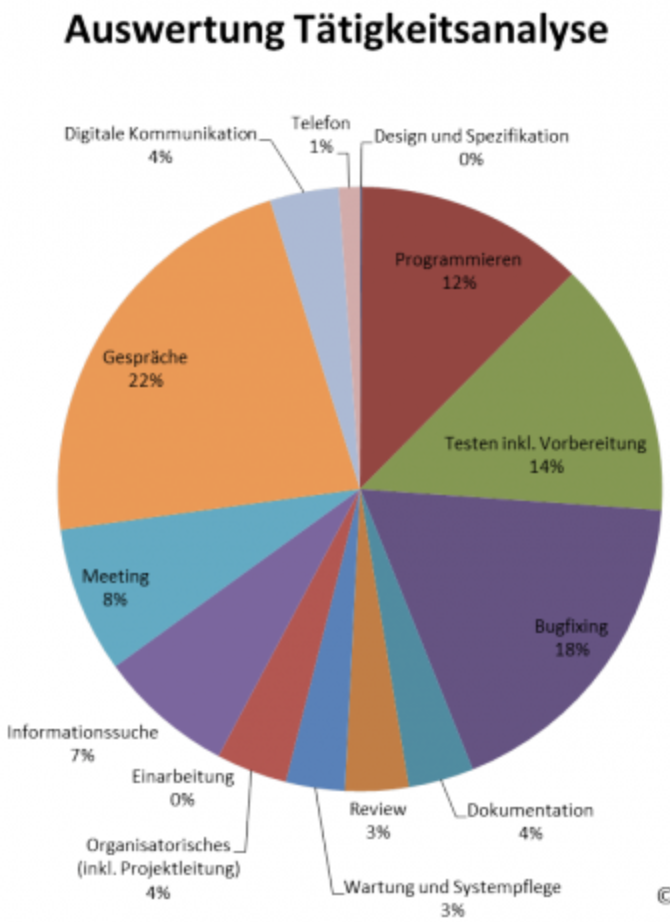
\includegraphics[width=3\marginparwidth]{auswertung.png}
    \caption{\label{fig:auswertungen}Beispielhafte Auswertung von Tätigkeiten in einem agilen Softwareprojekt \cite{Voigt:2015aa}}
\end{marginfigure}
\textbf{Persönlichen Daten in Review-Tools:} \newline
Diese Frage hat sich damit befasst, ob die Befragten Wert auf die Existenz von persönlichen Daten in Review-Tools (vgl. GitHub oder Gerrit) legen und falls ja, in was für einem Umfang sie diese benötigen bzw. nutzen. Für fünf der insgesamt sieben Befragten war es wichtig, einen Benutzernamen in
Review-Tools vorzufinden. Begründet wurde dies durch die allgemeine Möglichkeit der Zuordnung und der Identifikation eines Ansprechpartners im Falle von auftretenden Fragen und Wünschen und zum Einholen von Feedback in Bezug auf den verfassten Code. Drei Befragte, wovon sich bereits drei den Benutzernamen
gewünscht haben, möchten zusätzlich Zeitstempel in Review-Tools vorfinden können und erklären diesen Wunsch durch die Möglichkeit der zeitlichen Zuordnung der einzelnen Reviews: \enquote{Wann wurde ein Review zu meinem Programmcode bzw. zu meinem Build durchgeführt und wie relevant ist dieses im Augenblick?}. Im Arbeitsalltag lässt
sich also aus den Aussagen der Befragten ableiten, dass eine Einschätzung über die Dringlichkeit und Relevanz über die potenziell geforderten Änderungen und Anpassungen im Review seitens der Stakeholder erfolgt. \newline
Die verbliebenen zwei Experten, welche keinen Wert auf persönliche Daten jeglicher Art in Review-Tools legen, begründen ihre Sichtweise dadurch, keine Reviews durchführen zu müssen bzw. keine Reviews zu erhalten oder benötigen in ihrem Arbeitsalltag lediglich Reviews zum Inhalt ihres Codes bzw. zum Fehlschlagen von Builds, ohne jegliche Zeitangaben. \newline \newline
\textbf{Persönlichen Daten in Administrationstools:} \newline
Hier sollten die Befragten angeben, ob in den verwendeten Tools zur Administration persönliche Daten in Form von Zeitstempeln, Benutzernamen o.Ä. existieren. Die Befragten haben hierbei als Administrationstools angegeben, beispielsweise Jenkins als CI-Tool, SpringBoot als Framework oder einfache Kommunikationstools wie Slack und Microsoft-Teams (und insbesondere dessen Kalenderfunktion)
einzusetzen. \newline Im Prinzip sind sich alle Befragten einig, sowohl Benutzernamen, als auch Zeitstempel in Administrationstools zu benötigen und im Arbeitsalltag auch regelmäßig miteinzubeziehen. Um eine allgemeine Funktion von internen Kommunikationstools (zur eindeutigen Identifikation, mit welcher Person kommuniziert wird) zu gewährleisten und bei Builds anhand ihrer Zeitstempel (Startzeit und Dauer)
und dem Autor bei Fehlschlag nachvollziehen und einen Ansprechpartner identifizieren zu können, werden hier als Gründe angegeben. Lediglich ein Experte hat angegeben, in SpringBoot auf den Einsatz von persönlichen Daten jeglicher Form verzichten zu können, da diese bisher im eingesetzten SpringBoot ohnehin nicht existent waren. \newline \newline
\textbf{Detailgrad von Tickets in Ticketverwaltungstools:} \newline
In Ticketverwaltungstools (vgl. Jira\sidenote{Entwicklungstool zur agilen Softwareentwicklung, vgl. Atlassian \url{https://www.atlassian.com/de/software/jira}} oder Redmine\sidenote{Open-Source-Applikation für Projektmanagement, vgl. Redmine \url{https://www.redmine.org}}) kommen sogenannte \enquote{Issues} zum Einsatz. Damit werden die Tickets bezeichnet, welche z.T. von Kunden, aber auch von Mitarbeitern eines Softwareentwicklungsunternehmens selbst erstellt werden. Mit diesen werden beispielsweise auftretende Fehler in jeglicher Form gemeldet, Verbesserungs- bzw. Änderungswünsche angegeben
oder eine andere Aufgabenstellung festgehalten. \newline Dadurch ist es möglich, dass Mitarbeiter und Kunden einsehen, nachverfolgen und Kommentare zu den Tickets hinzufügen können, welche Probleme aufgetreten sind, welche Wünsche (z.B. von einer Applikation) gefordert sind oder welche Informationen zu einem bestimmten Thema relevant sind. Da ein grundlegendes Verständnis beim
Anlegen eines solchen Issue-Tickets gewährleistet sein muss, haben alle Befragten auch angegeben, eine ausführliche Issue-Beschreibung zu benötigen. In dieser befindet sich i.d.R. der Inhalt des Tickets (\enquote{Was genau muss getan werden?}, der Status (\enquote{Wie weit fortgeschritten ist diese Aufgabe?}, ein Zeitstempel (\enquote{Wann wurde diese Aufgabe erstellt?} 
und die Angabe eines Ticket-Erstellers und -Beauftragten (\enquote{Von wem wurde diese Aufgabe angelegt und wer soll diese bearbeiten?}, wobei diese bei sechs Befragten in Form eines Benutzernamen auftritt und beim verbliebenen als Vor- und Nachname. \newline Zusätzlich dazu wünschen alle sieben Experten, dass Benutzernamen und Zeitstempel in diesen vermerkt sind. Dies begründet ein 
Experte dadurch, dass die Lebensdauer eines Tickets stark variieren und z.T. nach mehreren Jahren und zweistelliger Anzahl von \enquote{Assignees} (Derzeitiger Beauftragte für die Bearbeitung des Tickets) weiterhin existieren kann und die Übersicht ohne diese verloren ginge - schließlich könne man so nicht nachverfolgen, welche Person zu welchem Datum bzw. zu welcher Uhrzeit 
was bearbeitet habe und dies für die Bearbeitung dieser Tickets erforderlich sei. \newline \newline
\textbf{Interesse an persönlichen daten in editierten Issues:} \newline \label{comments}
Ticketverwaltungstools bieten häufig die Möglichkeit, eigenen, verfassten Text, also in Kommentaren oder in der Beschreibung der Tickets, hinterher zu editieren. Zu diesem Aspekt wurden die Experten befragt, ob ein Interesse, von welcher Person zu welcher Zeit etwas (im Nachgang) editiert wurde, vorhanden sei. \newline Hier haben sechs Befragte angegeben, Benutzernamen, Zeitstempel und die ursprüngliche Nachricht
angezeigt bekommen zu wollen. Der Grund hierfür liegt erneut bei der Nachvollziehbarkeit von verfassten Kommentaren oder der Ticketbeschreibung, da es häufig vorkommt, dass Kommentare aufeinander oder auf die Beschreibung aufbauen und eine nachträgliche Änderung den Kontext dieser erschweren könnte. Vor allem bei \enquote{schwierigen Themen} sei dies häufig der Fall. Dabei reicht es drei der
fünf Experten nicht aus, lediglich einen Vermerk auf einen editierten Beitrag zu erhalten - diese wünschen sich zusätzlich, den ursprünglichen Beitrag, die Uhrzeit und den Benutzernamen, vom Verantwortlichen der Änderungen, angezeigt zu bekommen, da auf diese Art und Weise relevante Informationen aus den Änderungen gewonnen werden können (\enquote{Warum hat diese Person zu diesem Zeitpunkt diesen Beitrag
editiert?}). \newline Einer der sechs Experten, welche sich für editierte Beiträge interessieren, hat angegeben, keine Historie einsehen zu können und sich aufgrund dessen nicht für diese zu interessieren, weswegen eine einfache Anzeige, dass ein Beitrag editiert wurde (bspw. in Form eines einfachen Stempels oder Symbols), ausreichen würde. \newline \newline
\textbf{Tatsächliche Aufbewahrungsdauer von Log-Dateien:}\newline \label{logs}
Da ein überwiegender Anteil der Befragten von über 85\% (vgl. Tabelle \ref{tab:generaldata}) angegeben haben, Log-Dateien aktiv zu nutzen, ist es für den weiteren Verlauf der Analyse erforderlich, die tatsächliche Aufbewahrungsdauer der genutzten Log-Dateien 
im Unternehmen zu spezifizieren. Hier haben alle Befragten angegeben, dass alle Log-Dateien in der Regel für eine unbegrenzte bzw. unbestimmte Dauer aufbewahrt werden. Die Stakeholder haben zudem meist keine Kenntnis über die genaue Aufbewahrungsdauer und 
beziehen sich bei ihrer Aussage auf die Existenz von alten Log-Dateien (über 5 Jahre). \newline Die Ausnahme dieser Regel betrifft manuell durchgeführte Bereinigungen von Speicher und eingeleitete Löschungen spezifischer Log-Dateien: Bei einem Befragten kam es vor,
dass das System einen Absturz erlitten hat, welche die Log-Dateien unbenutzbar werden ließen, wohingegen bei einem anderen der Serverspeicher geleert werden musste und dieses Vorgehen sämtliche Log-Dateien gelöscht hat. \newline Aus diesen Aussagen lässt sich 
ableiten, dass ein Vorgehen zur automatisierten Löschung von Log-Dateien bei den Befragten bisher keine Anwendung gefunden hat. \newline \newline
\textbf{Mögliche Verarbeitungsinteressen von persönlichen Daten in anderen Unternehmen:} \newline
Im Rahmen dieser Frage ist es relevant gewesen, die Ansichten der Experten zu möglichen Verarbeitungsinteressen von persönlichen Daten in anderen Unternehmen einzuholen. Dadurch ist es möglich, ein allgemeines Bild von Softwareentwicklungsunternehmen im Ganzen zu erhalten, falls die Ansichten der Stakeholder sich als deckungsgleich zeigen sollten. \newline In der Tat haben etwa 57\% (vier der sieben Befragten) angegeben,
dass sie sich vorstellen können, wie Unternehmen die Arbeitszeiten der einzelnen Angestellten nachverfolgen können. Schließlich könne man einsehen, welche Person zu welcher Uhrzeit einen Commit bereitgestellt hat (durch Präsenz des Zeitstempels und Benutzernamens), wer im Kommunikationstool anwesend ist (Online-Status, z.B. in Microsoft Teams) oder wer zu welcher Uhrzeit auf E-Mails reagiert bzw. geantwortet hat, behaupten die Stakeholder.
Aus diesen gesammelten Daten eine Arbeitszeiten-Statistik anzulegen, sei nur einen kleinen Schritt von diesem Aspekt fortgeführt. Durch diesen Punkt könne man gebuchte Arbeitszeiten nachprüfen, korrigieren oder ggf. weglassen, da dies durch die Kontrolle redundant werden würde. \newline
Zusätzlich hat ein Befragter angegeben, sich vorstellen zu können, dass Ressourcenmanagement betrieben werden könne: Durch die Einsicht in die Arbeits- bzw. Anwesenheitszeiten der einzelnen Angestellten, hat dieser Befragte behauptet, könne man vorhandene Ressourcen (wie z.B. eingeschaltete Server, Computer oder Strom im Allgemeinen) sparen, indem man diese, abhängig zu den genannten Zeiten, zur Verfügung stellt. Das jeweilige Unternehmen
könne so laufende Betriebskosten sparen, was im eigenen Interesse liegen würde.

\subsection{Kategorien mit einer Präferenz für die Privatsphäre} \label{privacy}
\textbf{Persönlichen Daten in Log-Dateien:} \newline
Dieser Punkt befasst sich mit dem allgemeinen Interesse an persönlichen Daten, welche in Form von Benutzernamen, Zeitstempeln, IDs etc. in Log-Dateien sämtlicher Art auftreten können. Hier haben die Befragten einstimmig
entschieden, kein Interesse an diesen zu haben und ein mögliches Entfernen in der Zukunft willkommen zu heißen. Es wurde lediglich angegeben, dass in bestimmten Fällen (Zusammenarbeit an einem Projekt, 
in Testfällen von Code, Servern oder Applikationen oder auf Anfrage) eine Nachverfolgung auf Wunsch eines Kunden oder eines Auftrags erfolgen muss. \newline Für die Befragten ist es nur wichtig, den Ablauf und auftretende Fehler 
von Servern, Applikationen oder Code im Allgemeinen nachverfolgen zu können - ein Interesse an bestimmten Personen oder Zeitstempeln ist nicht vorhanden, weswegen in dieser Kategorie die Privatsphäre über der Nutzerfreundlichkeit
steht. \newline \newline
\textbf{Bevorzugte Aufbewahrungsdauer von Log-Dateien:} \newline
Als Weiterleitung der Frage über die tatsächliche Aufbewahrungsdauer von Log-Dateien in Kapitel \ref{noprivacy} wurden in dieser Kategorie die Experten dazu angehalten, ihre persönliche Präferenz zur Dauer anzugeben. Hier haben alle 
Befragten angegeben, eine temporäre Aufbewahrungsdauer zu bevorzugen. Begründet wurde dies dadurch, dass Log-Dateien nur für wenige bestimmte Fälle, welche i.d.R. relativ neu sind (<2 Monate), benötigt werden und über diesen Zeitraum
hinaus redundant werden.

\section{Kategorien mit abweichenden Ergebnissen} \label{noclearresult}
Dieses Kapitel befasst sich mit der verbliebenen Kategorie, in welcher Aussagen zu Sichtweisen seitens der einzelnen Stakeholder getroffen wurden, die sich zu keiner eindeutigen Aussage zusammenfassen lassen und dementsprechend separat 
behandelt werden müssen. Als ein abweichendes Ergebnis wird dabei bezeichnet, dass bei sieben Befragten weniger als 28\% (entspricht: maximal zwei Befragte besitzen die selbe Ansicht) die selbe Sichtweise zu einer Kategorie haben und somit kein einstimmiges Ergebnis vorliegt. \newline \newline
\textbf{Sonstige relevante Daten aus der Sicht der Stakeholder:} \newline
Zu diesem Aspekt wurden die Experten befragt, ob ihnen sonstige, für sie relevante, Daten im Arbeitsalltag in den Sinn kommen. Diese Frage ist insofern relevant, da hierdurch potenziell neue Aspekte offenbart werden können, welche im Arbeitsalltag eines Stakeholders Anwendung finden. Dementsprechend
haben lediglich drei der sieben Befragten eine individuelle Vorstellung wiedergeben können. \newline Da diese sich selbst aber voneinander unterscheiden und keine gemeinsame Kategorie ausfindig gemacht werden konnte, werden diese im Kapitel mit den Kategorien mit abweichenden Ergebnissen behandelt: Für einen Befragten ist es beispielsweise wichtig, den Umfang eines Commits in DevOps-Tools einsehen zu können. Das bedeutet, dass eine Unterscheidung, ob es sich bei einem Commit nun um eine \enquote{kleine Fehlerbehebung}
oder eine \enquote{große Implementierung eines neuen Features} handelt, durchgeführt werden kann. Dies sei vor allem zur Einschätzung des Arbeitsaufwandes und der Forderungen zur Herangehensweise an die Aufgabe selbst notwendig. \newline \newline 
Ein weiterer Experte hat zusätzlich angegeben, die Überprüfung der Anwesenheit der Angestellten vor Ort würde einen wichtigen Bestandteil seines Arbeitsalltages darstellen. Dadurch könne dieser einen Überblick haben, wer gerade in unmittelbarer Nähe anzusprechen ist und seiner Arbeit nachgeht. \newline Als letzten Aspekt wurde die Aussage getroffen, dass die Commit-Frequenz der eigenen Kollegen für diesen Befragten eine große Rolle spielt: Dadurch könne er, im Falle eines Merge-Requests (Anfrage zum Einbinden eines Commits in das Hauptverzeichnis), einschätzen, wieviel dieser im jeweiligen Commit an Änderungen bzw. Anpassungen zu erwarten hat.
Laut eigener Angabe sei es im eigenen Softwareentwicklungsunternehmen üblich, dass unterschiedliche Entwickler unterschiedliche Commit-Frequenzen aufweisen. Manche stellen deutlich größere, aber seltener Commits bereit, als manche andere, welche viele, kleine Commits als angemessen empfinden. Anhand dieser Information könne der Befragte den Commit wohl angemessener beurteilen.

\section{Vorgeschlagene Alternativen} \label{alternatives}
\textbf{Temporäre Zeitstempel in DevOps-Tools}: \newline
Zusätzlich zur gewünschten Auflösung von Zeitstempeln in DevOps-Tools haben vier der sieben Befragten angegeben, eine temporäre Lebensdauer der Zeitstempel zu bevorzugen, da diese nach einer bestimmten Zeit an Relevanz verlieren würden. Abhängig sei dies beispielsweise durch die Anzahl der zuletzt erfolgreich durchgeführten Builds, einem bestimmten Zeitraum x oder nach vollendeter Lebensdauer eines Tickets. 
Die Befragten haben dabei Bezug zum eigenen Arbeitsalltag genommen, in welchem die Zeitstempel ohne festgelegte Dauer bestehen bleiben würden und nur nach einer manuell durchgeführten Löschung des übergeordneten Speicherpunktes (z.B. eines abgelaufenen Builds, veralteten Commits etc.) verschwinden würden. \newline \newline
\textbf{Temporäre Aufbewahrungsdauer von Log-Dateien in Abhängigkeit von Faktor xy:} \newline
Zu der Frage, welche Länge zur Aufbewahrung von Log-Dateien seitens der Stakeholder bevorzugt werde, haben sechs von sieben Experten angegeben, eine temporäre Aufbewahrung von Log-Dateien willkommen zu heißen. Diese könne anhand der Lebensdauer von Projekten, der Lebensdauer von Programmcode, den letzten x Builds, einer festgelegten Zeit (z.B. zwei Wochen/Monaten)
oder der Existenz von gemeldeten Fehlern deklariert werden. In der Regel sind sich die Befragten einig, eine Dauer von maximal wenigen Monaten zu bevorzugen. \newline Diese Sichtweisen stellen einen Gegensatz zur tatsächlichen Aufbewahrungsdauer von Log-Dateien in Softwareentwicklungsunternehmen dar, welche in Kapitel \ref{noprivacy} angesprochen werden. Begründet wird dieser Vorschlag
durch die kaum vorhandene Nutzung von alten (z.B. älter als zwei Monate) Log-Dateien im Arbeitsalltag der Stakeholder.
